\documentclass[12pt]{beamer}
\usetheme{metropolis}

\newenvironment{code}{\ttfamily}{\par}

\title{systemd}
\subtitle{The standard Linux init system}

\begin{document}
\metroset{titleformat frame=allcaps}

\maketitle

\section{Introduction}

\begin{frame}{What is an init system?}
  An init system is the first userspace process (PID 1) started in a UNIX-like system. It handles:

  \begin{itemize}
  \item Starting system processes and services to prepare the environment
  \item Adopting and ``reaping'' orphaned processes
  \end{itemize}
\end{frame}

\begin{frame}{Classical init systems}
  Init systems before systemd - such as SysVinit - were very simple.

  \begin{itemize}
  \item Services and processes to run are organised into ``init scripts''
  \item Scripts are linked to specific runlevels
  \item Init system is configured to boot into a runlevel
  \end{itemize}

\end{frame}

\section{systemd}

\begin{frame}{Can we do better?}
  \begin{itemize}
  \item ``legacy'' init systems have a lot of drawbacks
  \item Apple is taking a different approach on OS X
  \item Systemd project was founded to address these issues
  \end{itemize}
\end{frame}

\begin{frame}{Systemd design goals}
  \begin{itemize}
  \item Expressing service dependencies
  \item Monitoring service status
  \item Enable parallel service startups
  \item Ease of use
  \end{itemize}
\end{frame}

\begin{frame}{Systemd - the basics}
  \begin{itemize}
  \item No scripts are executed, only declarative units
  \item Units have explicit dependencies
  \item Processes are supervised
  \item cgroups are utilised to apply resource limits
  \item Service logs are managed and centrally queryable
  \item Much more!
  \end{itemize}
\end{frame}

\begin{frame}{Systemd units}
  Units specify how and what to start. Several types exist:
  \begin{code}
    \small
    \begin{columns}[T,onlytextwidth]
      \column{0.5\textwidth}
      \begin{itemize}
      \item systemd.service
      \item systemd.target
      \item systemd.timer
      \item systemd.path
      \item systemd.socket
      \end{itemize}
      \column{0.5\textwidth}
      \begin{itemize}
      \item systemd.device
      \item systemd.mount
      \item systemd.swap
      \item systemd.slice
      \end{itemize}
    \end{columns}
  \end{code}
\end{frame}


\begin{frame}{Resource management}
  Systemd utilises Linux \texttt{cgroups} for resource management, specifically CPU, disk I/O and memory usage.

  \begin{itemize}
  \item Hierarchical setup of groups makes it easy to limit resources for a set of services
  \item Units can be attached to a \texttt{systemd.slice} for controlling resources for a group of services
  \item Resource limits can also be specified directly in the unit
  \end{itemize}
\end{frame}

\begin{frame}{journald}
  Systemd comes with an integrated log management solution, replacing software such as \texttt{syslog-ng}.
  \begin{itemize}
  \item All process output is collected in the journal
  \item \texttt{journalctl} tool provides many options for querying and tailing logs
  \item Children of processes automatically log to the journal as well
  \item \textbf{Caveat:} Hard to learn initially
  \end{itemize}
\end{frame}

\begin{frame}{Systemd tooling}
  A variety of CLI-tools exist for managing systemd systems.
  \begin{code}
    \begin{itemize}
    \item systemctl
    \item journalctl
    \item systemd-analyze
    \item systemd-cgtop
    \item systemd-cgls
    \end{itemize}
  \end{code}

  Let's look at some of them.
\end{frame}

\section{Demo}

\section{Controversies}

\begin{frame}{Systemd criticism}
  Systemd has been heavily criticised, usually focusing around a few points:
  \begin{itemize}
  \item Feature-creep: Systemd absorbs more and more other services
  \end{itemize}
\end{frame}

\begin{frame}{Systemd criticism}
  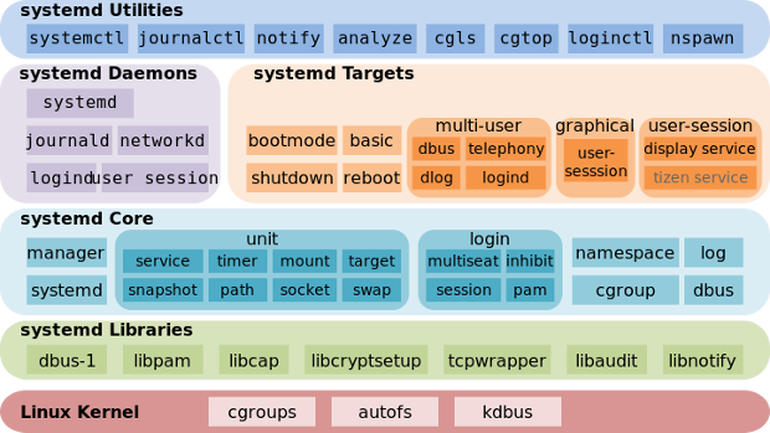
\includegraphics[keepaspectratio=true,width=\textwidth]{systemdcomponents.png}
\end{frame}

\begin{frame}{Systemd criticism}
  Systemd has been heavily criticised, usually focusing around a few points:
  \begin{itemize}
  \item Feature-creep: Systemd absorbs more and more other services
  \item Opaque: systemd's inner workings are harder to understand than old \texttt{init}
  \item Unstable: development is quick and breakage happens
  \end{itemize}
\end{frame}

\begin{frame}{Systemd adoption}
  Systemd was initially adopted by RedHat (and related distributions).

  It spread quickly to others, for example ArchLinux.

  Debian and Ubuntu were the last major players who decided to adopt it, but not without drama.
\end{frame}

\section{Questions?}

\end{document}
